\documentclass[12pt, a4paper]{article}

% ── Encoding and fonts ────────────────────────────────────────────────────────
\usepackage[utf8]{inputenc}
\usepackage[T1]{fontenc}
\usepackage{lmodern}

% ── Page layout ───────────────────────────────────────────────────────────────
\usepackage[top=2.5cm, bottom=2.5cm, left=2.5cm, right=2.5cm]{geometry}
\usepackage{setspace}
\onehalfspacing

% ── Mathematics ───────────────────────────────────────────────────────────────
\usepackage{amsmath}
\usepackage{amssymb}

% ── Units and numbers ─────────────────────────────────────────────────────────
\usepackage{siunitx}
\sisetup{
    detect-all,
    range-phrase = {--},
    range-units  = single,
}

% ── Tables ────────────────────────────────────────────────────────────────────
\usepackage{booktabs}
\usepackage{array}

% ── Figures ───────────────────────────────────────────────────────────────────
\usepackage{graphicx}
\usepackage{float}

% ── Hyperlinks ────────────────────────────────────────────────────────────────
\usepackage[
    colorlinks = true,
    linkcolor  = blue,
    citecolor  = blue,
    urlcolor   = blue,
]{hyperref}

% ── References ────────────────────────────────────────────────────────────────
\usepackage[
    round,
    authoryear,
    sort&compress,
]{natbib}

% ── Angles ────────────────────────────────────────────────────────────────────
\usepackage{gensymb}   % provides \degree, \ang needs siunitx ≥ 3 or textcomp

% ── Misc ──────────────────────────────────────────────────────────────────────
\usepackage{microtype}
\usepackage{xcolor}
\usepackage{enumitem}

% ─────────────────────────────────────────────────────────────────────────────
\title{%
    \textbf{Supplementary Material}\\[0.5em]
    \large Afforestation as a Carbon Dioxide Removal Technology in PyPSA-Eur:\\
    Methodology for Spatial and Temporal Sequestration Rates
}
\author{Alberto Alamia \and [co-authors]}
\date{\today}
% ─────────────────────────────────────────────────────────────────────────────

\begin{document}

\maketitle
\tableofcontents
\newpage

% =============================================================================
\subsection{Afforestation as a Carbon Dioxide Removal Technology}
\label{sec:afforestation_methodology}

Afforestation was first introduced in PyPSA-eur in \cite{Fernandes2026} as a spatially resolved carbon dioxide removal (CDR) technology. The implementation requires two inputs per network node: (i)~the
available land area from CORINE land cover, (ii)~a CO$_2$ sequestration rate
in \si{tCO_2 / (ha a)}. Here is introduced a more accurate approach to the calculation of the CO2 sequestration rates, which ensure consistency with EU LULUCF legislation, and provides a sub-annual temporal profile distributing the uptake across calendar months. This section describes
the derivation of both CO$_2$ sequestration rates and temporal profiles from publicly available European forest inventory and remote-sensing data.

% =============================================================================
\subsubsection{Annual Sequestration Rate: Pilli et al.\ Yield Table Library}
\label{sec:affo_rate}

\paragraph{Data source.}
The sequestration rates are derived from the JRC forest growth library compiled by \citet{Pilli2024}, which provides age-class-resolved volume and increment
curves for 222~forest types across 25~EU Member States (EU-27 excluding Cyprus
and Malta). The library is distributed via Zenodo
\cite{Pilli2024Zenodo} described in \cite{Pilli2024} and contains three key datasets:

\begin{itemize}[leftmargin=2em]
    \item \textbf{Standing stock} (m$^3$\,ha$^{-1}$): net merchantable volume
          under bark by 10-year age class for even-aged stands.
    \item \textbf{Net Annual Increment} (NAI, m$^3$\,ha$^{-1}$\,yr$^{-1}$):
          merchantable volume growth rate by age class, harmonised across
          countries using species-specific correction factors for bark,
          branches, top, and stump components.
    \item \textbf{Biomass Conversion and Expansion Factors} (BCEF,
          t$_\text{DM}$\,m$^{-3}$): age-class-resolved factors converting
          merchantable volume to total aboveground dry biomass, derived from
          species-specific allometric equations \citep{Boudewyn2007}.
\end{itemize}

The data are classified by country, administrative region (mostly NUTS-2),
forest type (leading species), management type, and management strategy
(even-aged or uneven-aged). The original NFI reference years span 1992--2018,
with most countries reporting data from the 2005--2015 period.

\paragraph{Why this method.}
The yield-table-based approach was preferred over remote-sensing biomass
products \citep[e.g.][]{Avitabile2024} because
it: (i)~provides region- and species-specific growth trajectories calibrated
against national forest inventories; (ii)~is consistent with the carbon
accounting methodology used in the EU Carbon Budget Model (EU-CBM-HAT,
\citealt{Grassi2018}); and (iii)~yields a single rotation-averaged rate that
is directly applicable as a long-run average CDR potential, which is arguably the parameter required for modeling of the energy system. We applied the method only to productive forests assuming that new afforestation or reforestation project will fall within the categories: management types ``H'', ``HP'', ``HS'', and ``MAN'', while  coppice, non-productive, and protected forests are excluded. The original method in \cite{Fernandes2026} derived the CO2 sequestration rates from the standing above-ground biomass density (tDM / ha) of all forests, assuming a single Europe-wide averaged parameter as a single duration peak-growth-phase of forests.

% =============================================================================
\subsubsection{Rotation-Averaged Sequestration Rate}
\label{sec:affo_mai}

For new afforestation, we compute a \emph{rotation-averaged} Mean Annual
Increment (MAI), which represents the long-term average CO$_2$ uptake rate
over a full forest rotation. This approach avoids the overestimation that
would result from using peak-growth-phase increment values, and is consistent
with the EU LULUCF accounting framework \citep{EU2018841, EU2023839}.

For each combination of forest type~$f$, region~$r$, and management type~$m$,
the computation proceeds as follows.

\paragraph{Step 1: Determine optimal rotation age.}
The rotation age $T^*$ is defined as the age at which the volumetric MAI is
maximised:
\begin{equation}
    T^* = \arg\max_{T \geq T_\text{min}} \frac{V(T)}{T}
    \label{eq:rotation_age}
\end{equation}
where $V(T)$ is the standing stock (m$^3$\,ha$^{-1}$) at age~$T$ and
$T_\text{min} = \SI{25}{yr}$ is a minimum rotation age imposed to avoid
numerical artefacts at very young age classes. The age classes are reported
at 10-year intervals with midpoints at 5, 15, 25, \ldots, \SI{195}{yr}.

\paragraph{Step 2: Compute volumetric MAI.}
The rotation-averaged volumetric MAI is:
\begin{equation}
    \text{MAI}_\text{vol} = \frac{V(T^*)}{T^*}
    \quad [\text{m}^3\,\text{ha}^{-1}\,\text{yr}^{-1}]
    \label{eq:mai_vol}
\end{equation}

\paragraph{Step 3: Convert volume to CO$_2$.}
The volumetric MAI is converted to a CO$_2$ sequestration rate using the BCEF
at the rotation age, the IPCC carbon fraction, and a root-to-shoot expansion:
\begin{equation}
    \text{MAI}_{\text{CO}_2} = \text{MAI}_\text{vol}
        \times \text{BCEF}(T^*)
        \times C_f
        \times \frac{M_{\text{CO}_2}}{M_C}
        \times (1 + R)
    \quad [\text{tCO}_2\,\text{ha}^{-1}\,\text{yr}^{-1}]
    \label{eq:mai_co2}
\end{equation}
where $\text{BCEF}(T^*)$ is the Biomass Conversion and Expansion Factor at
the rotation age (t$_\text{DM}$\,m$^{-3}$), converting merchantable volume
to total aboveground biomass; $C_f = 0.5$ is the carbon fraction of dry
biomass \citep{IPCC2006}; $M_{\text{CO}_2}/M_C = 44/12$ is
the molecular mass ratio of CO$_2$ to carbon; and $R = 0.25$ is the
root-to-shoot ratio accounting for belowground biomass
\citep{IPCC2006, Mokany2006}.

\paragraph{Step 4: Regional aggregation.}
For each NUTS-2 region, the sequestration rate is computed using a two-step
procedure that reflects both the IPCC methodology for afforestation accounting
and European biodiversity guidelines for mixed-species plantings.

In the first step, an equal-weight average of the rotation-averaged MAI is
computed separately for coniferous and broadleaved species groups:
\begin{equation}
    \overline{\text{MAI}}^{g}_{\text{CO}_2, r}
    = \frac{1}{|F^{g}_r|} \sum_{f \in F^{g}_r} \text{MAI}_{\text{CO}_2, f, r}
    \qquad g \in \{\text{con},\, \text{broad}\}
    \label{eq:nuts2_group}
\end{equation}
where $F^{g}_r$ is the set of productive forest types of group $g$ present in
region~$r$.
Only even-aged, productive high-forest stands are included (management types
``H'', ``HP'', ``HS'', and ``MAN'').

In the second step, the two group means are blended with equal weight,
representing a 50\,\% coniferous / 50\,\% broadleaved planting mix:
\begin{equation}
    \overline{\text{MAI}}_{\text{CO}_2, r}
    = \frac{1}{2}\,\overline{\text{MAI}}^{\text{con}}_{\text{CO}_2, r}
    + \frac{1}{2}\,\overline{\text{MAI}}^{\text{broad}}_{\text{CO}_2, r}
    \label{eq:nuts2_agg}
\end{equation}
If only one species group has data in a region, that group's mean is used
directly.

The 50/50 con/broad split is grounded in European silvicultural practice.
The EU Biodiversity Strategy 2030 requires that new forests meet strict
biodiversity criteria and promotes diverse, mixed-species stands
\citep{EC2020BiodiversityStrategy}.
Most EU member-state forest laws mandate a minimum broadleaved fraction of
20--30\,\% in new plantings (e.g.\ Germany's \emph{Bundeswaldgesetz});
a 50/50 split satisfies this threshold with margin and represents a
conservative, biodiversity-compatible assumption.
The approach is consistent with the \citet{IPCC2006} Good Practice Guidance
for afforestation and reforestation, which prescribes the rotation-averaged
MAI as the basis for estimating long-run mean annual carbon accumulation of
a newly established stand.
Within each species group, equal weighting across forest types is used as an
approximation in the absence of NFI-derived species-area data at NUTS-2
resolution.

% =============================================================================
\subsubsection{Spatial Coverage: Mapping to All NUTS-2 Regions}
\label{sec:affo_nuts2_coverage}

The modeling approach introduced in \cite{Fernandes2026} requires sequestration rates for all the NUTS-2 region in the PyPSA-eur model which are later applied to the available land for afforestation computed from the CORINE LAND COVER dataset. The input library \cite{Pilli2024Zenodo} covers only 23 countries and uses a mix of NUTS-2, NUTS-1, and
national-level regions. Gaps arise for countries outside the library
(e.g.\ Norway, Switzerland, Turkey, the Western Balkans) as well as for
specific NUTS-2 regions within covered countries (e.g.\ small island regions
or city-states that fall below the spatial resolution of the NFI data).

To ensure full spatial coverage, a cascade of fallback strategies is applied
in the following order:

\begin{enumerate}[leftmargin=2em]
    \item \textbf{Direct NUTS-2 match:} the NUTS-2 region code in \cite{Pilli2024Zenodo} corresponds
          exactly to a NUTS-2 identifier.
    \item \textbf{NUTS-1 propagation:} a three-character Pilli region code is
          matched to all child NUTS-2 regions sharing the same NUTS-1 prefix
          (e.g.\ \texttt{DEA} propagated to \texttt{DEA1}--\texttt{DEA5}).
    \item \textbf{Country-level propagation:} for countries where the input
          library reports a single national value at NUTS-0 level,
          that value is applied uniformly to all NUTS-2 regions within the
          country.
    \item \textbf{Distance-based neighbour mean:} for remaining unassigned
          regions, the mean of all NUTS-2 regions whose boundary lies within
          \SI{100}{km} is used. A \SI{100}{km} threshold was chosen to
          capture meaningful sea crossings---the Strait of Dover
          (${\approx}\SI{34}{km}$), the Irish Sea (${\approx}\SI{70}{km}$),
          and similar crossings in the Adriatic and Baltic---without
          introducing long-range links such as Scotland to Norway
          (${\approx}\SI{300}{km}$). The step is iterated until no further
          regions can be filled, propagating values continuously inward from
          continental anchors through island chains and isolated regions such
          as the British Isles.
    \item \textbf{Country mean:} the mean of all resolved NUTS-2 regions
          within the same country, used for genuinely isolated island regions
          (e.g.\ the Canary Islands, Madeira, Azores).
    \item \textbf{Mediterranean analogue (Malta, Cyprus):} \texttt{MT00} and
          \texttt{CY00} are assigned the value of \texttt{EL43} (Crete), the
          geographically and climatically closest region with a direct Pilli
          estimate.
\end{enumerate}


The source of each assigned value is recorded on zenodo (future) \cite{Alamia_Zenodo2026} for reproducibility.

% =============================================================================
\subsubsection{Temporal Weighting: Monthly Sequestration Profiles}
\label{sec:affo_temporal}

To represent the seasonality of forest carbon uptake,
the annual sequestration rate is disaggregated into monthly increments using
observed Gross Primary Production (GPP) data as a proxy for the seasonal
pattern of photosynthetic activity. GPP is the total amount of carbon fixed
by plants through photosynthesis per unit area and time; it is highest in
summer when light and temperature favour growth, and near zero in winter in
temperate and boreal regions. It therefore serves as a direct observational
indicator of when forests are actively sequestering carbon throughout the year.

\paragraph{Data source.}
Monthly weighting factors are derived from the FluxCom RS+METEO ensemble
\citep{Jung2020}, which provides daily global GPP estimates at \ang{0.5}
spatial resolution using a machine-learning upscaling of eddy covariance flux
tower observations, driven by ERA5 meteorological reanalysis and MODIS
remote-sensing inputs. The specific dataset used is:

\begin{quote}
\small
\texttt{GPP.RS\_METEO.FP-ALL.MLM-ALL.METEO-ERA5.720\_360.daily.\{year\}.nc}\\[2pt]
Unit: \si{gC\,m^{-2}\,day^{-1}} \quad
Resolution: \ang{0.5} global \quad
Years: 2010--2012 (${\approx}\SI{3.6}{GB}$ total)\\
Source: \citet{Jung2020}; data accessed via anonymous FTP at
\texttt{ftp.bgc-jena.mpg.de} (Max Planck Institute for Biogeochemistry,
Jena, Germany).
\end{quote}

Three years (2010--2012) are used to construct a stable climatological
seasonal cycle while limiting data volume. The ERA5-forced ensemble was
selected over the purely remote-sensing-driven product because ERA5 provides
continuous, gap-free meteorological forcing consistent with the climate data
used elsewhere in PyPSA-Eur.

\paragraph{Why GPP as a temporal proxy.}
GPP is the appropriate proxy for the seasonal distribution of afforestation
carbon uptake because: (i)~it directly measures photosynthetic carbon
assimilation, which drives biomass accumulation; (ii)~it naturally captures
the phenological seasonality of temperate and boreal forests, including
growing-season onset and senescence; and (iii)~it is available at the spatial
and temporal resolution required for NUTS-2 aggregation across Europe. 

\paragraph{Step 1: Monthly climatology.}
For each of the three downloaded annual files, the daily GPP field is clipped
to the European geographical region, and the monthly mean climatological is  computed by averaging all daily values
within each month across all three years:
\begin{equation}
    G_m(\lambda, \phi)
    = \frac{1}{N_m} \sum_{y=2010}^{2012} \sum_{d \in \mathcal{D}_{m,y}}
      \text{GPP}(\lambda, \phi, d)
    \quad [\text{gC\,m}^{-2}\,\text{day}^{-1}]
    \label{eq:gpp_climatology}
\end{equation}
where $\mathcal{D}_{m,y}$ is the set of days in month~$m$ of year~$y$ and
$N_m$ is the total number of averaging days. This yields a 12-layer
climatological field at \ang{0.5} resolution.

\paragraph{Step 2: Zonal aggregation to NUTS-2.}
Each \ang{0.5} grid cell is assigned to a NUTS-2 region by a
point-in-polygon test using the cell centroid and the NUTS-2013 polygon
boundaries \citep{Eurostat2013NUTS}. For regions containing at least one
grid cell, the monthly GPP is computed as the mean of all assigned cells
with finite, positive values:
\begin{equation}
    \bar{G}_{m,r}
    = \frac{1}{\left|\mathcal{C}_r^+\right|}
      \sum_{c \in \mathcal{C}_r^+} G_m(\lambda_c, \phi_c)
    \quad [\text{gC\,m}^{-2}\,\text{day}^{-1}]
    \label{eq:gpp_zonal}
\end{equation}
where $\mathcal{C}_r^+$ is the set of grid cells assigned to region~$r$
with $G_m > 0$. For very small regions (city-states, small islands) that
contain no grid-cell centre, the value of the nearest grid cell (by centroid
distance) is used as a fallback.

\paragraph{Step 3: Normalisation to monthly weights.}
For each NUTS-2 region, the 12 monthly GPP values are normalised to obtain
dimensionless weights $w_{m,r}$ that sum to unity:
\begin{equation}
    w_{m,r} = \frac{\bar{G}_{m,r}}{\displaystyle\sum_{m'=1}^{12} \bar{G}_{m',r}},
    \qquad \sum_{m=1}^{12} w_{m,r} = 1
    \label{eq:gpp_weights}
\end{equation}
Months in which GPP is zero or not recorded (e.g.\ winter months in northern
regions where the signal falls below the detection threshold) are treated as
zero flux; if all 12 months are missing, the fallback cascade below is
triggered instead of re-normalisation.

For regions where no valid GPP signal is available in any month, the same
fallback cascade as in Section~\ref{sec:affo_nuts2_coverage} is applied:
\begin{enumerate}[leftmargin=2em]
    \item Mean profile of NUTS-2 regions within \SI{100}{km} (EPSG:3035),
          iterated until stable, so that values propagate across sea crossings
          (e.g.\ southern England from northern France).
    \item Mean profile of all resolved regions in the same country.
    \item Uniform profile: $w_{m,r} = 1/12$ for all months (last resort).
\end{enumerate}

\paragraph{Step 4: Monthly sequestration rates.}
The monthly CO$_2$ sequestration rate for region~$r$ is obtained by
multiplying the annual rate by the monthly weight:
\begin{equation}
    \text{Rate}_{m,r}
    = w_{m,r} \times \overline{\text{MAI}}_{\text{CO}_2,\, r}
    \quad [\text{tCO}_2\,\text{ha}^{-1}\,\text{month}^{-1}]
    \label{eq:monthly_rate}
\end{equation}
By construction,
$\sum_{m=1}^{12} \text{Rate}_{m,r} = \overline{\text{MAI}}_{\text{CO}_2,\, r}$,
preserving the annual carbon budget. These monthly rates are passed to
PyPSA-Eur as the time-varying efficiency of the afforestation CDR component.

% =============================================================================
\subsubsection{Consistency with EU Policy Frameworks}
\label{sec:affo_policy}

The rotation-averaged MAI is consistent with the EU LULUCF Regulation
\citep{EU2018841, EU2023839}, which requires gross-net accounting of removals
on afforested land over a 20--30~year transition period.

\paragraph{CRCF accounting.}
Regulation~(EU)~2024/3012 \citep{EU20243012} established the EU Carbon
Removal Certification Framework; the afforestation methodology was issued as
a draft delegated act on 22~January~2026. Three points are relevant here.

\textit{(i) Activity period:} 30~years (no renewal), followed by 40~years of
monitoring --- consistent with the PyPSA-Eur technology lifetime.

\textit{(ii) Harvest is permitted} provided trees are replanted and no net
stock reduction occurs (§1.1.3.2(h)(i)); a net decrease triggers a
\emph{reversal} and credit invalidation. The MAI concept is therefore
appropriate: it already represents the long-run average annual stock increase
of a managed stand that includes the harvest--replant cycle.

\textit{(iii) Discounts.} Credits equal the net stock increase times
$(1-\mathrm{UNC})$, where UNC is a mandatory uncertainty deduction (min.\
10\%). Operators also contribute a risk-rate share to a buffer pool after
each audit; these units expire at end of monitoring (permanent discount).
Risk rates from Table~7 of the draft are 8--17\,\% for broadleaf/mixed
forests at low-to-medium disturbance. The net fraction of gross MAI that
becomes usable credits is:
\begin{equation}
  \eta_\text{CRCF} = (1 - \text{UNC})(1 - r_\text{risk})
  \label{eq:crcf_efficiency}
\end{equation}
giving $\eta_\text{CRCF}\approx0.75$--$0.83$ for typical European conditions.
The remaining gross stock decomposes exactly as net certified stock
($\eta_\text{CRCF}$), buffer reserve ($(1-\mathrm{UNC})\,r$), and a
harvest/safety margin (UNC) --- carbon never credited and therefore
extractable without reversal; the three sum to unity by construction.
In PyPSA-Eur, $\eta_\text{CRCF}$ is the \texttt{Link} \texttt{efficiency},
set via \texttt{afforestation[crcf\_efficiency]} (default~0.80).
Figure~\ref{fig:mai_crcf} illustrates all three components.

\begin{figure}[htbp]
  \centering
  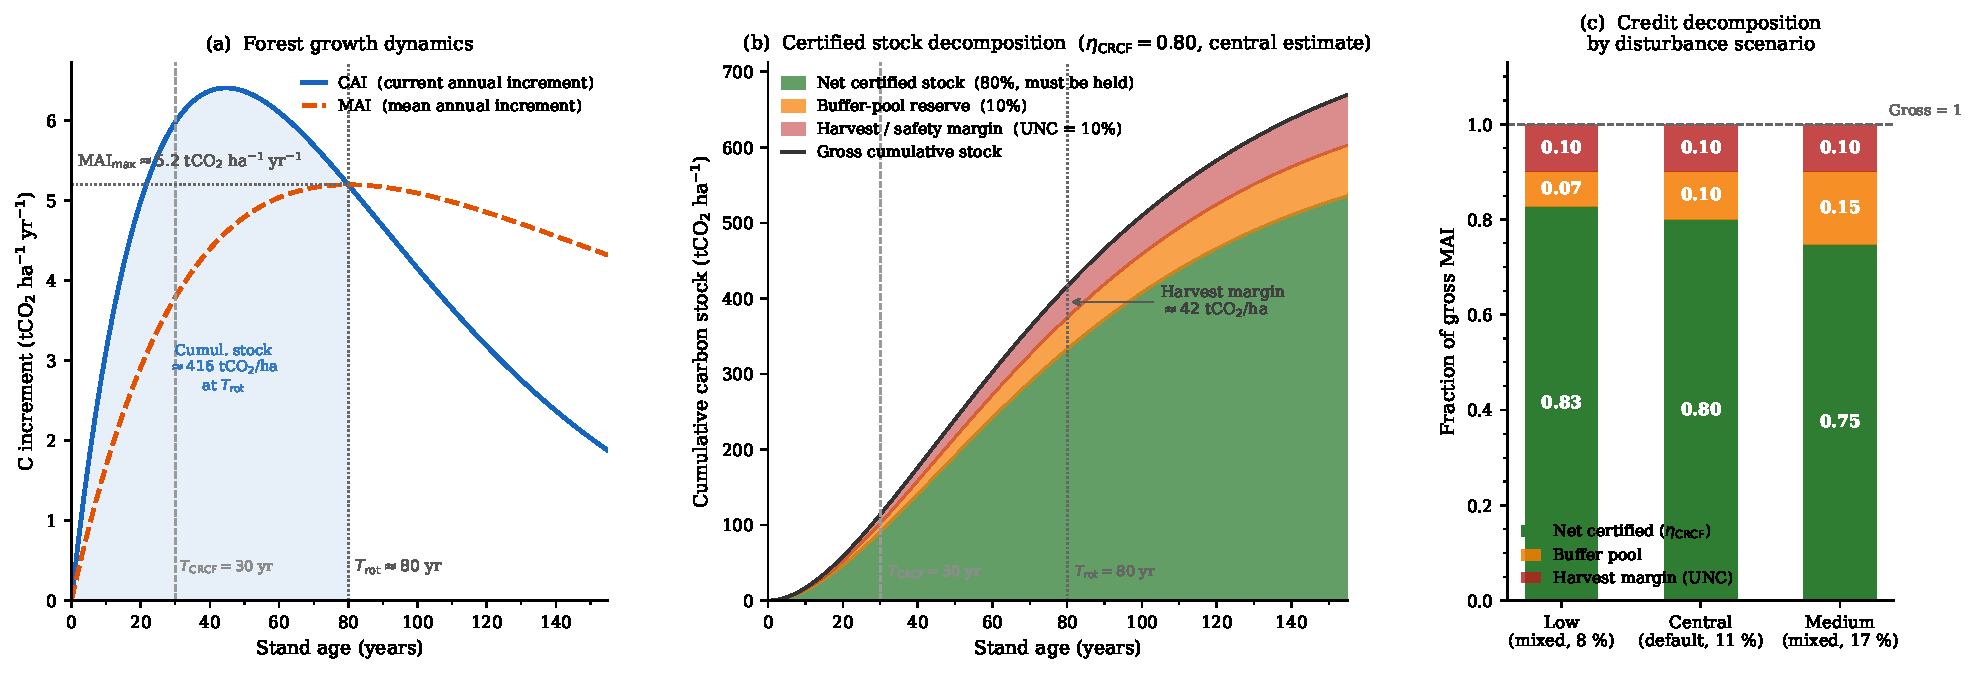
\includegraphics[width=\textwidth]{figures/mai_crcf_explained.pdf}
  \caption{%
    \textbf{Forest growth dynamics, certified stock, and CRCF credit breakdown.}
    \textit{(a)} CAI (blue) and MAI (dashed orange) for a representative
    European managed forest ($T_\text{rot}\approx80$\,yr,
    MAI$_\text{max}\approx5.2$\,tCO$_2$ ha$^{-1}$ yr$^{-1}$;
    EU median from \citealt{Pilli2024Zenodo}); dashed line: 30-yr CRCF
    activity period.
    \textit{(b)} Gross cumulative stock decomposed into net certified stock
    (green), buffer-pool reserve (orange), and harvest/safety margin (red,
    = UNC fraction, extractable without triggering reversal).
    Central estimate: $\eta_\text{CRCF}=0.80$, UNC$=10\,\%$, $r=11\,\%$.
    \textit{(c)} Same fractions for three disturbance scenarios
    (Table~7, draft delegated act, 22~Jan.~2026).}
  \label{fig:mai_crcf}
\end{figure}

% =============================================================================
\subsubsection{PyPSA-Eur implementation}
\label{sec:affo_pypsa}

Each network node has a \texttt{Store} on a dedicated \texttt{co2 afforestation}
bus, linked to \texttt{co2 atmosphere} via an extendable \texttt{Link}.
Storage capacity (\texttt{e\_nom\_max}) is set by the CORINE land area and
annual sequestration rate; capital cost is annualised over a 30-year lifetime.
The \texttt{Link} \texttt{efficiency} equals $\eta_\text{CRCF}$
(Eq.~\ref{eq:crcf_efficiency}), so only the certified fraction of gross
sequestration reaches the storage bus. Both methods are available via
\texttt{afforestation[potential\_type]} (\texttt{``density''}: \citealt{Fernandes2026};
\texttt{``growth''}: this work; see \url{https://github.com/BertoGBG/pypsa-eur/tree/a_CDRs}).

\paragraph{Seasonal dispatch profile.}
In growth mode, \texttt{p\_min\_pu}$(t) =$ \texttt{p\_max\_pu}$(t)$ forces
the \texttt{Link} to follow the GPP-derived seasonal profile exactly,
leaving the optimiser only the capacity $p_\text{nom}$ to choose:
\begin{equation}
    p_{\min,r}(t) = p_{\max,r}(t)
    = w_{m(t),\,r} \cdot \frac{T_\text{year}}{H_{m(t)}}
    \label{eq:ppu}
\end{equation}
where $w_{m,r}$ is the normalised GPP weight for node~$r$ in month~$m$
(Eq.~\ref{eq:gpp_weights}) and $H_m$ is the number of snapshot hours in
month~$m$. The factor $T_\text{year}/H_m$ preserves the annual budget:
$\sum_t p_\text{nom}\,\bar{p}_r(t) = p_\text{nom}\,T_\text{year}$,
equivalent to fixed monthly budgets proportional to $w_{m,r}$.
The \texttt{Store} \texttt{e\_nom\_max}~$= \Pi_r$ (tCO$_2$ yr$^{-1}$)
implicitly caps the link: $p_\text{nom} \leq \Pi_r/T_\text{year}$.
The optimiser therefore chooses the fraction of land to deploy; the
seasonal shape is fixed by the profile.

% =============================================================================
\subsubsection{Results and Validation}
\label{sec:affo_results}

The computed rotation-averaged sequestration rates range from
\SIrange{2.1}{12.6}{tCO_2\per ha\per yr} across 114~NUTS-2 regions with
direct Pilli data, with a European median of \SI{5.2}{tCO_2\per ha\per yr}
and mean of \SI{5.5}{tCO_2\per ha\per yr}. These values are consistent with
the \SIrange{5}{15}{tCO_2\per ha\per yr} range reported for temperate European
afforestation in the literature \citep{Nabuurs2013, Avitabile2024}.

As a validation case, the five Danish NUTS-2 regions yield rates of
\SIrange{3.9}{5.8}{tCO_2\per ha\per yr}, with a national average of
approximately \SI{5.1}{tCO_2\per ha\per yr}. This is in reasonable
agreement with the \SI{6.5}{tCO_2\per ha\per yr} estimated by
\citet{Fernandes2026} for a 60\%~conifer / 40\%~broadleaf species mix;
the difference is attributable to the equal-weight species averaging used
here versus an area-weighted approach giving greater weight to
higher-productivity conifer species.

Table~\ref{tab:affo_rates_sample} reports a selection of regional rates.

\begin{table}[htbp]
\centering
\caption{Rotation-averaged CO$_2$ sequestration rates for selected NUTS-2
regions. $\bar{T}$: mean rotation age across forest types included;
$n$: number of productive forest types.}
\label{tab:affo_rates_sample}
\sisetup{round-mode=places, round-precision=1}
\begin{tabular}{
    l
    l
    S[table-format=2.1]
    S[table-format=3.0]
    S[table-format=2.0]
}
\toprule
{Country} & {NUTS-2} &
{Rate [\si{tCO_2\,ha^{-1}\,yr^{-1}}]} &
{$\bar{T}$ [yr]} & {$n$} \\
\midrule
Austria   & AT21  & 6.8  & 47  & 8  \\
Belgium   & BE20  & 6.9  & 34  & 7  \\
Czechia   & CZ01  & 5.2  & 48  & 4  \\
Denmark   & DK01  & 5.8  & 39  & 7  \\
Denmark   & DK05  & 3.9  & 39  & 7  \\
Finland   & FI1A  & 2.5  & 25  & 3  \\
France    & FRF1  & 5.4  & 27  & 6  \\
Germany   & DE2   & 7.2  & 34  & 8  \\
Ireland   & IE    & 7.1  & 33  & 6  \\
Italy     & ITH5  & 5.6  & 40  & 14 \\
Poland    & SL    & 5.9  & 31  & 8  \\
Romania   & RO21  & 6.0  & 28  & 9  \\
Sweden    & SE11  & 4.3  & 100 & 4  \\
Sweden    & SE33  & 2.1  & 33  & 4  \\
\bottomrule
\end{tabular}
\end{table}

Figure~\ref{fig:affo_monthly_nodes} shows the resulting monthly sequestration
rates aggregated to the 50-node PyPSA-Eur network. The seasonal pattern is
consistent with expectations: rates are near zero across most of Europe in
winter (December--February), rise sharply in spring, peak in June--July for
temperate and boreal nodes, and decline again in autumn. Southern nodes
(Iberian Peninsula, Italy, Greece) exhibit a broader active season and a
relatively flatter seasonal cycle, reflecting the year-round photosynthetic
activity captured by the FluxCom GPP climatology in Mediterranean climates.
The highest monthly rates (${\approx}\SI{1.5}{tCO_2\,ha^{-1}\,month^{-1}}$)
occur in central European nodes during peak summer, consistent with the
high rotation-averaged MAI values reported for Germany, Austria, and Ireland
in Table~\ref{tab:affo_rates_sample}.

\begin{figure}[htbp]
    \centering
    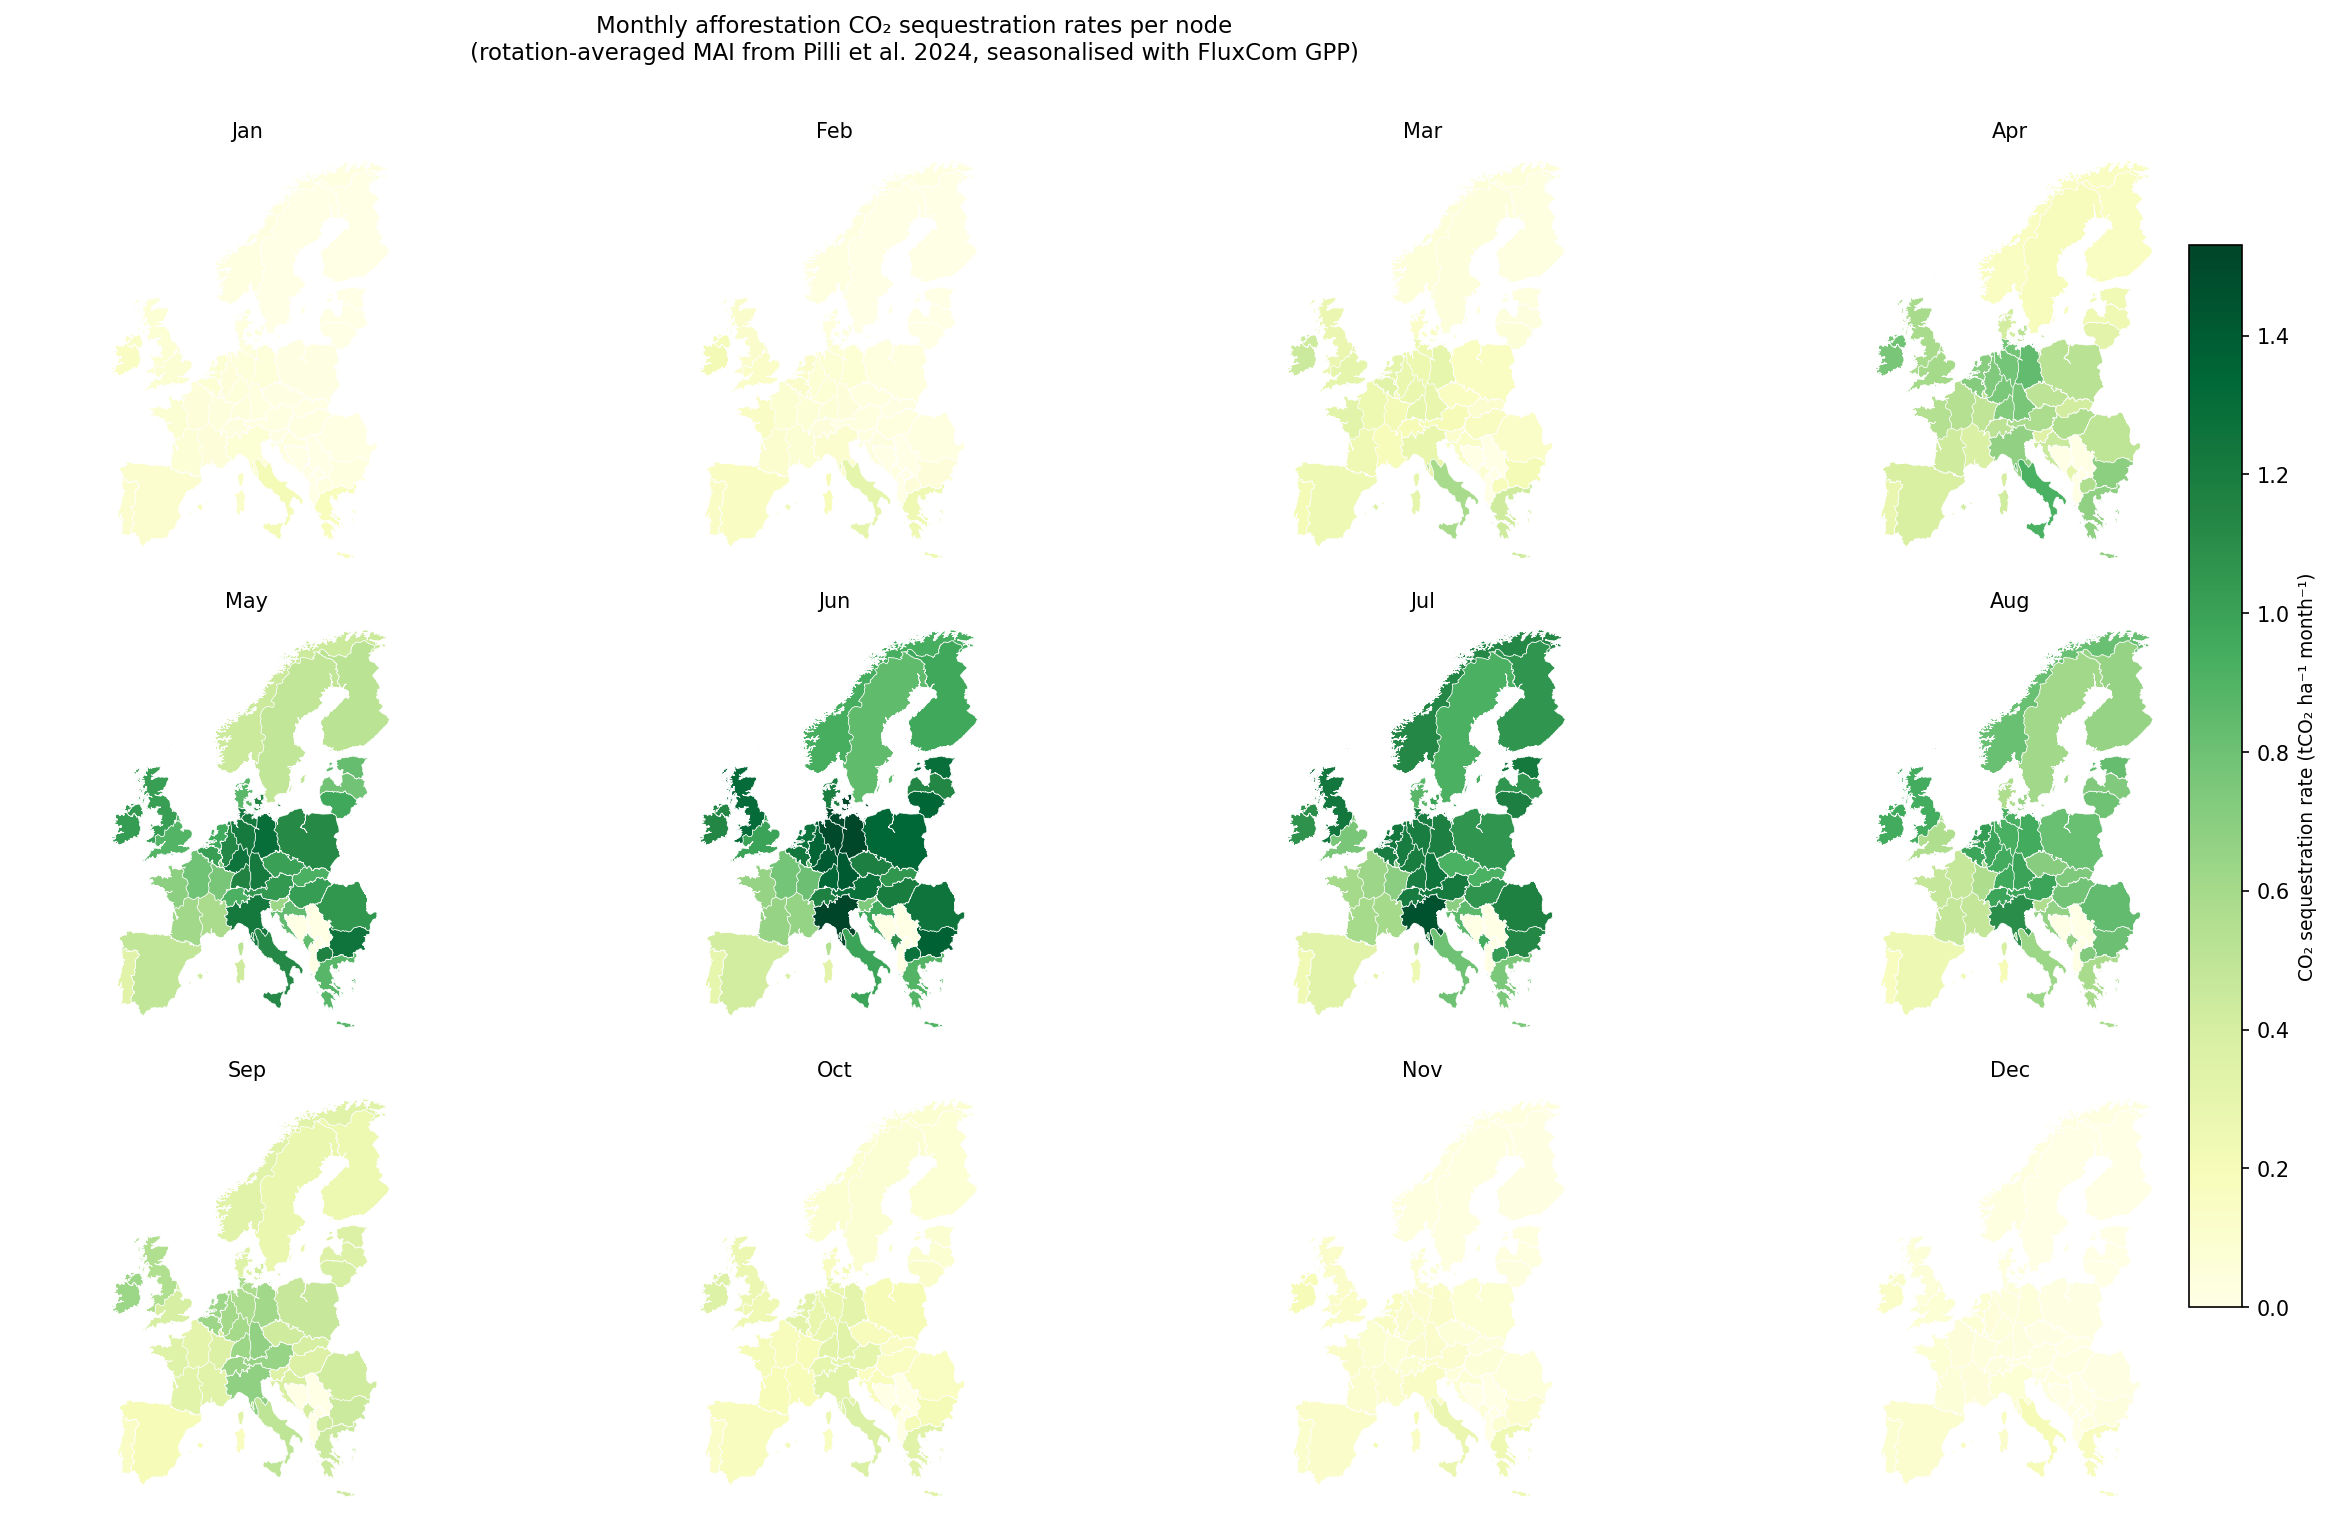
\includegraphics[width=\textwidth]{figures/afforestation_potentials_s_50.png}
    \caption{Monthly afforestation CO$_2$ sequestration rates per network node
    for a 50-node PyPSA-Eur configuration
    [\si{tCO_2\,ha^{-1}\,month^{-1}}].
    Each panel shows one calendar month; node colours reflect the product of
    the rotation-averaged MAI (Section~\ref{sec:affo_mai}) and the
    GPP-derived monthly weight $w_{m,r}$ (Eq.~\ref{eq:monthly_rate}).
    The strong north--south gradient in summer activity and the near-zero
    winter rates in boreal and continental nodes are clearly visible.
    Generated by \texttt{build\_afforestation\_potentials.py} in the
    PyPSA-Eur \texttt{afforestation} branch.}
    \label{fig:affo_monthly_nodes}
\end{figure}

% =============================================================================
\newpage
\bibliographystyle{apalike}
\bibliography{references}

\end{document}
